\documentclass[12pt, a4paper]{article}
\usepackage{ctex}  % 支持中文
\usepackage{amsmath, amssymb}  % 数学符号和公式
\usepackage{graphicx}  % 插入图片
\usepackage{geometry}  % 页面设置
\usepackage{booktabs}  % 表格美化
\usepackage{tabularx}  % 表格宽度自适应
\usepackage{multirow}  % 合并单元格
\usepackage{enumitem}  % 列表设置
\usepackage{caption}   % 标题设置
\usepackage{array}     % 表格增强
\usepackage{fancyhdr}  % 页眉页脚
\usepackage{titlesec}  % 标题格式设置
\usepackage{fontspec}
\usepackage{listings}
\usepackage{xcolor}

\usepackage[
  backend=bibtex,
  style=gb7714-2015,   % 使用中国国标格式,适合中文论文
  sorting=none         % 按引用顺序排序
]{biblatex}

\addbibresource{references.bib} % 参考文献配置

% 页面设置
\geometry{left=2.5cm, right=2.5cm, top=2.5cm, bottom=2.5cm}

% 重定义section格式为居中
\titleformat{\section}{\centering\Large\bfseries}{\thesection}{1em}{}
\titleformat{\subsection}{\normalsize\bfseries}{\thesubsection}{1em}{}
\titleformat{\subsubsection}{\normalsize\bfseries}{\thesubsubsection}{1em}{}

% 表格表头格式
\renewcommand{\thetable}{\arabic{section}.\arabic{table}}

% 设置表格标题格式:左对齐,中文带"表"字,表题加粗
\captionsetup[table]{
  labelsep=space,
  labelformat=simple,
  textfont=bf,
  labelfont=bf,
  name=表
}

% 图片编号格式
\renewcommand{\thefigure}{\arabic{section}-\arabic{figure}}

% 设置图片标题格式
\captionsetup[figure]{
  labelsep=space,
  labelformat=simple,
  textfont=bf,     
  labelfont=bf, 
  position=bottom,  
  name=图
}

% 修改公式编号格式
\renewcommand{\theequation}{\thesection-\arabic{equation}}

% 参考文献格式
\makeatletter
\renewcommand\@biblabel[1]{[#1]}
\makeatother

% 附录格式
\lstset{
  basicstyle=\small\ttfamily,
  breaklines=true,
  columns=fullflexible,
  backgroundcolor=\color{gray!10},
  frame=single,
  rulecolor=\color{black!30},
  commentstyle=\color{green!50!black},
  keywordstyle=\color{blue},
  stringstyle=\color{red},
  numbers=left,
  numberstyle=\tiny\color{gray},
  numbersep=5pt
}


\begin{document}

% 标题部分
\begin{center}
\LARGE\textbf{中国股市投资组合优化协方差矩阵的估计}

\vspace{1cm}
\large 计金220 22011854 高菻铠
\end{center}

\noindent \textbf{摘要:} 本研究探究了不同协方差矩阵估计方法在中国A股市场投资组合优化中的应用与效果。基于2010-2021年十个申万一级行业指数月度收益率数据,研究实现并比较了样本协方差矩阵、常量估计法、三因子模型估计法、压缩估计法及指数加权移动平均法五种估计方法。采用滚动窗口技术,研究在最小风险与最大效用两种优化目标下构建的投资组合表现。实证结果表明,结构化方法尤其是三因子模型与压缩估计法在降低噪声与保留风险结构间取得了理想平衡,表现出较高稳健性。投资组合权重动态变化反映了市场风险结构的时变特性,其中最大效用组合展现出更为均衡的权重分配与更优的风险调整收益。行业配置呈现出周期性与结构性特征,防御性行业权重相对稳定,而周期性行业权重波动较大。研究验证了协方差矩阵估计方法对投资组合绩效的实质性影响,并为投资者根据市场环境与个体风险偏好选择适当估计方法提供了实证依据。

\section{文献综述}

金融投资组合优化是现代金融理论的重要组成部分,而协方差矩阵的估计作为投资组合构建过程中的关键环节,直接影响投资策略的有效性。随着对冲基金等另类投资工具的兴起,如何准确估计资产收益的协方差矩阵成为当前研究的热点问题。

\citet{sun2019covariance}针对对冲基金分布复制模型中协方差估计问题进行了深入研究。该研究指出,传统的指数加权移动平均(EWMA)方法虽然被广泛应用于对冲基金复制,但存在计算量大和完全依赖样本数据的明显缺陷。为克服这些局限,作者提出了两种改进方法:基于因子模型的协方差估计和基于收缩模型的协方差估计,并引入了预处理技术来消除金融数据中的噪声影响。

在研究背景方面,\citet{sun2019covariance}首先回顾了对冲基金复制策略的发展历程。自2003年以来,分布复制法作为对冲基金复制技术之一受到学界关注,随后经历了多次改进。作者以Takahashi模型为基础,将研究重点放在波动率矩阵的计算过程中如何确定协方差矩阵上,提出了替代传统指数移动加权平均法的新方法。

在理论构建方面,\citet{sun2019covariance}详细阐述了Takahashi模型的数学基础。该模型假设金融市场是完全市场,资产价格满足特定的随机微分方程,通过状态价格密度过程确定最小初始投入的动态投资组合。作者证明,在该框架下,动态投资组合的计算归结为无风险利率、漂移率和波动率三个参数的计算,其中波动率矩阵与协方差矩阵存在一一对应关系。

针对协方差矩阵估计,\citet{sun2019covariance}提出了三种方法:一是传统的指数加权移动平均法,二是基于单因子市场模型的因子估计法,三是基于线性组合的收缩估计法。特别地,基于因子模型的估计通过引入市场因子降低了数据维度,而基于收缩的估计则通过设定最优收缩强度提高了估计的稳健性。此外,作者还采用修剪均值滤波器进行金融数据去噪预处理,以降低市场噪声的干扰。

在实证分析方面,\citet{sun2019covariance}以道琼斯瑞士信贷对冲基金指数为复制目标,使用美元兑日元汇率和日元黄金作为复制工具,构建了基于不同协方差估计方法的动态投资组合。通过对2006年1月3日至2007年1月3日期间数据的分析,研究发现:(1)经过去噪处理后,复制策略的波动率显著降低,表明去噪能有效减小策略风险;(2)在所有协方差估计方法中,基于收缩的协方差矩阵估计得到的复制策略拥有最高的平均日对数收益率和最低的标准差,即最高的单位风险价格;(3)当样本数量较少时,基于因子模型的估计并未展现出降维方面的优势。

\citet{sun2019covariance}的研究表明,在对冲基金分布复制过程中,协方差矩阵的估计方法对复制策略的风险收益特性具有显著影响。其中,基于收缩的协方差估计方法表现最佳,数据去噪预处理则能进一步提高策略的风险调整收益。这些发现为投资组合优化和对冲基金复制策略的实际应用提供了重要参考。

\section{数据与方法}

\subsection{数据描述}
本研究使用了10个申万一级行业指数2010至2021年的月度收益率数据,包括农林牧渔、采掘、化工、钢铁、有色金属、电子、家用电器、食品饮料、房地产和医药生物。数据来源于Tushare平台。经过数据清洗后,每个行业指数包含约132个有效观测点。行业指数月收益率计算公式为:

\begin{equation}
R_{t}^i = \frac{P_{t}^i - P_{t-1}^i}{P_{t-1}^i}
\end{equation}

其中,$P_t^i$ 为第 $t$ 月第 $i$ 个行业指数的收盘点位。

此外,我们通过Tushare获取了同期的上证指数(000001.SH)月度收益率数据,作为市场组合收益率的代理变量,并获取了Fama-French三因子模型数据,包括市场风险溢价因子(MKT)、规模因子(SMB)和价值因子(HML)。为了计算超额收益率,我们使用了行业收益率减去市场收益率的方法:

\begin{equation}
R_{excess,t}^i = R_{t}^i - R_{t}^{market}
\end{equation}

数据获取、清洗和收益率计算均通过Python中的Tushare、NumPy和Pandas等库实现。

\subsection{协方差矩阵估计方法}
在投资组合优化中,协方差矩阵的准确估计至关重要。本研究实现了五种不同的协方差矩阵估计方法,以较为全面地构建最优投资组合。

\subsubsection{样本方差-协方差矩阵估计}
最直接的方法是使用历史数据计算样本方差-协方差矩阵:

\begin{equation}
\hat{\Sigma}_{sample} = \frac{1}{T-1} \sum_{t=1}^{T} (R_t - \bar{R})(R_t - \bar{R})'
\end{equation}

其中,$R_t$ 是各资产在第 $t$ 期的超额收益率向量,$\bar{R}$ 是平均超额收益率向量,$T$ 是样本窗口长度(本研究设定为36个月)。

\subsubsection{常量估计法}
常量估计法保留了样本协方差矩阵的对角线元素(方差),但将非对角线元素(协方差)替换为使用平均相关系数计算的估计值:

\begin{equation}
\hat{\Sigma}_{constant,ij} = 
\begin{cases}
\hat{\sigma}_i^2, & \text{if } i = j \\
\bar{\rho} \cdot \hat{\sigma}_i \cdot \hat{\sigma}_j, & \text{if } i \neq j
\end{cases}
\end{equation}

其中,$\hat{\sigma}_i^2$ 是资产 $i$ 的样本方差,$\bar{\rho}$ 是所有资产对之间的平均相关系数。这种方法减小了协方差矩阵估计中的噪声影响。

\subsubsection{因子模型估计法}
本研究采用Fama-French三因子模型估计协方差矩阵。首先,对每个资产超额收益率进行如下回归:

\begin{equation}
R_t^i = \alpha^i + \beta_{MKT}^i \cdot MKT_t + \beta_{SMB}^i \cdot SMB_t + \beta_{HML}^i \cdot HML_t + \epsilon_t^i
\end{equation}

其中,$MKT_t$、$SMB_t$ 和 $HML_t$ 分别是市场、规模和价值因子的收益率,$\epsilon_t^i$ 是残差。然后,协方差矩阵估计为:

\begin{equation}
\hat{\Sigma}_{factor} = B \cdot \Omega \cdot B' + D
\end{equation}

其中,$B$ 是因子载荷矩阵,$\Omega$ 是因子协方差矩阵,$D$ 是残差协方差矩阵(通常假设为对角矩阵)。根据文献建议,我们还应用了偏差调整:

\begin{equation}
\hat{\Sigma}_{factor}^{adjusted} = B \cdot \Omega \cdot B' + \frac{T-2}{T-1} \cdot D
\end{equation}

\subsubsection{压缩估计法}
压缩估计法将样本协方差矩阵与一个结构化目标矩阵(本研究中选择对角矩阵)进行线性组合:

\begin{equation}
\hat{\Sigma}_{shrink} = (1-\rho) \cdot \hat{\Sigma}_{sample} + \rho \cdot \text{diag}(\hat{\Sigma}_{sample})
\end{equation}

其中,$\rho$ 是压缩强度参数,计算公式为:

\begin{equation}
\rho = \min \left( \frac{(1 - \frac{2}{n}) \text{tr}(\hat{\Sigma}_{sample}^2) + (\text{tr}\hat{\Sigma}_{sample})^2}{(T - \frac{2}{n}) \left( \text{tr}(\hat{\Sigma}_{sample}^2) - \frac{(\text{tr}\hat{\Sigma}_{sample})^2}{n} \right)}, 1 \right)
\end{equation}

其中,$n$ 是资产数量,$T$ 是样本窗口长度。

\subsubsection{指数加权移动平均估计法}
指数加权移动平均(EWMA)方法通过对历史数据进行指数衰减加权,使得近期数据在协方差矩阵估计中获得更高的权重:

\begin{equation}
\hat{\Sigma}_{EWMA} = \sum_{i=0}^{T-1} w_i R_{T-i} R_{T-i}'
\end{equation}

其中,权重 $w_i = (1-\lambda)\lambda^i / \sum_{j=0}^{T-1} \lambda^j$,$\lambda$ 是衰减因子(本研究中设置为0.94)。

\subsection{投资组合优化方法}
基于上述估计的协方差矩阵,我们实施了两种投资组合优化策略:最小化期望风险和最大化投资者效用。

\subsubsection{最小化期望风险的投资组合}
在目标收益率约束下,最小化投资组合方差的优化问题可表述为:

\begin{equation}
\begin{aligned}
\min_{w} \quad & w' \Sigma w \\
\text{s.t.} \quad & w' \mu = \mu_P \\
& w' \textbf{1} = 1 \\
& w_i \geq 0, \quad \forall i = 1, 2, \ldots, n
\end{aligned}
\end{equation}

其中,$w$ 是权重向量,$\Sigma$ 是协方差矩阵,$\mu$ 是期望收益率向量,$\mu_P$ 是目标组合收益率。在实际实现中,我们使用矩阵求解方法:

\begin{equation}
w^* = \Sigma^{-1} A' (A \Sigma^{-1} A')^{-1} b
\end{equation}

其中,$A = [\mu'; \textbf{1}']$,$b = [\mu_P; 1]$。

\subsubsection{最大化效用的投资组合}
假设投资者具有均值-方差效用函数:

\begin{equation}
U(w) = w' \mu - \frac{\gamma}{2} w' \Sigma w
\end{equation}

其中,$\gamma$ 是风险规避系数(本研究中设置为3)。最大化效用的优化问题为:

\begin{equation}
\begin{aligned}
\max_{w} \quad & w' \mu - \frac{\gamma}{2} w' \Sigma w \\
\text{s.t.} \quad & w' \textbf{1} = 1 \\
& w_i \geq 0, \quad \forall i = 1, 2, \ldots, n
\end{aligned}
\end{equation}

理论上,无约束最优解为 $w_{unconstrained} = \frac{1}{\gamma} \Sigma^{-1} \mu$。考虑权重和为1的约束后,最优解可表示为:

\begin{equation}
w^* = w_{unconstrained} + \lambda (\Sigma^{-1} \textbf{1})
\end{equation}

其中,$\lambda = \frac{1 - \textbf{1}' w_{unconstrained}}{\textbf{1}' \Sigma^{-1} \textbf{1}}$。

\subsection{投资组合表现评估}
本研究采用样本外回测方法评估投资组合表现。从2018年1月开始,使用过去36个月的滚动窗口数据估计协方差矩阵;随后基于最优化策略计算投资组合权重;持有该投资组合一个月,计算实际收益率;之后滚动前进一个月,重复上述过程,直至样本末期(2021年12月)。

对于优化后的投资组合,计算以下表现指标:
\begin{equation}
\begin{aligned}
\text{年化收益率} &= \overline{R}_p \times 12 \\
\text{年化波动率} &= \sigma_p \times \sqrt{12} \\
\text{夏普比率} &= \frac{\text{年化收益率}}{\text{年化波动率}}
\end{aligned}
\end{equation}

其中,$\overline{R}_p$ 是投资组合月均超额收益率,$\sigma_p$ 是投资组合月度收益率的标准差。

\subsection{方法实现}
上述所有方法均基于Python实现。数据获取通过Tushare API完成,数据处理和分析使用NumPy和Pandas库。协方差矩阵估计和投资组合优化使用SciPy的优化模块实现。对于可能出现的矩阵求逆问题,设计了回退机制,在矩阵接近奇异时采用数值优化方法。此外,利用Matplotlib和Seaborn进行数据可视化分析,展示不同估计方法下的协方差矩阵结构和投资组合权重演变。

\section{实证结果}

\subsection{协方差矩阵估计方法比较}

本研究基于2010-2021年中国A股市场10个行业指数的月度收益率数据,对不同协方差矩阵估计方法进行比较分析。实证研究采用滚动窗口法,使用36个月(3年)的历史数据估计协方差矩阵,并构建最优投资组合。研究期间为2018年1月至2021年12月,每月根据最新估计的协方差矩阵调整投资组合权重。表~\ref{tab:cov_methods}概述了本研究采用的五种协方差矩阵估计方法。

\begin{table}[htbp]
\centering
\caption{协方差矩阵估计方法对比}
\label{tab:cov_methods}
\begin{tabular}{lp{10cm}}
\toprule
\textbf{估计方法} & \textbf{基本原理与特点} \\
\midrule
样本方差-协方差矩阵 & 直接使用历史数据计算样本协方差,最为简单直接,但在高维数据下估计误差较大 \\
常量估计法 & 保留样本方差,但将协方差设为平均相关系数与样本标准差的乘积,降低估计噪声 \\
因子模型估计法 & 基于Fama-French三因子模型,将资产收益分解为系统性风险和特异性风险,通过因子载荷和因子协方差矩阵估计总体协方差 \\
压缩估计法 & 将样本协方差矩阵与结构化目标矩阵进行线性组合,通过文献公式(20)确定最优压缩系数 \\
指数加权移动平均法 & 对历史数据赋予时间衰减权重,近期数据权重更高,能更好捕捉市场风险动态变化 \\
\bottomrule
\end{tabular}
\end{table}

图~\ref{fig:cov_heatmap}展示了在2020年11月30日使用不同方法估计的协方差矩阵热力图。可以观察到,样本协方差矩阵元素波动较大,而常量估计法则过度平滑了相关结构。三因子模型和压缩估计法保留了主要风险结构,同时减少了估计噪声。特别是电子行业(801080)表现出较高的风险,在多种估计方法中均有体现。

\begin{figure}[htbp]
\centering
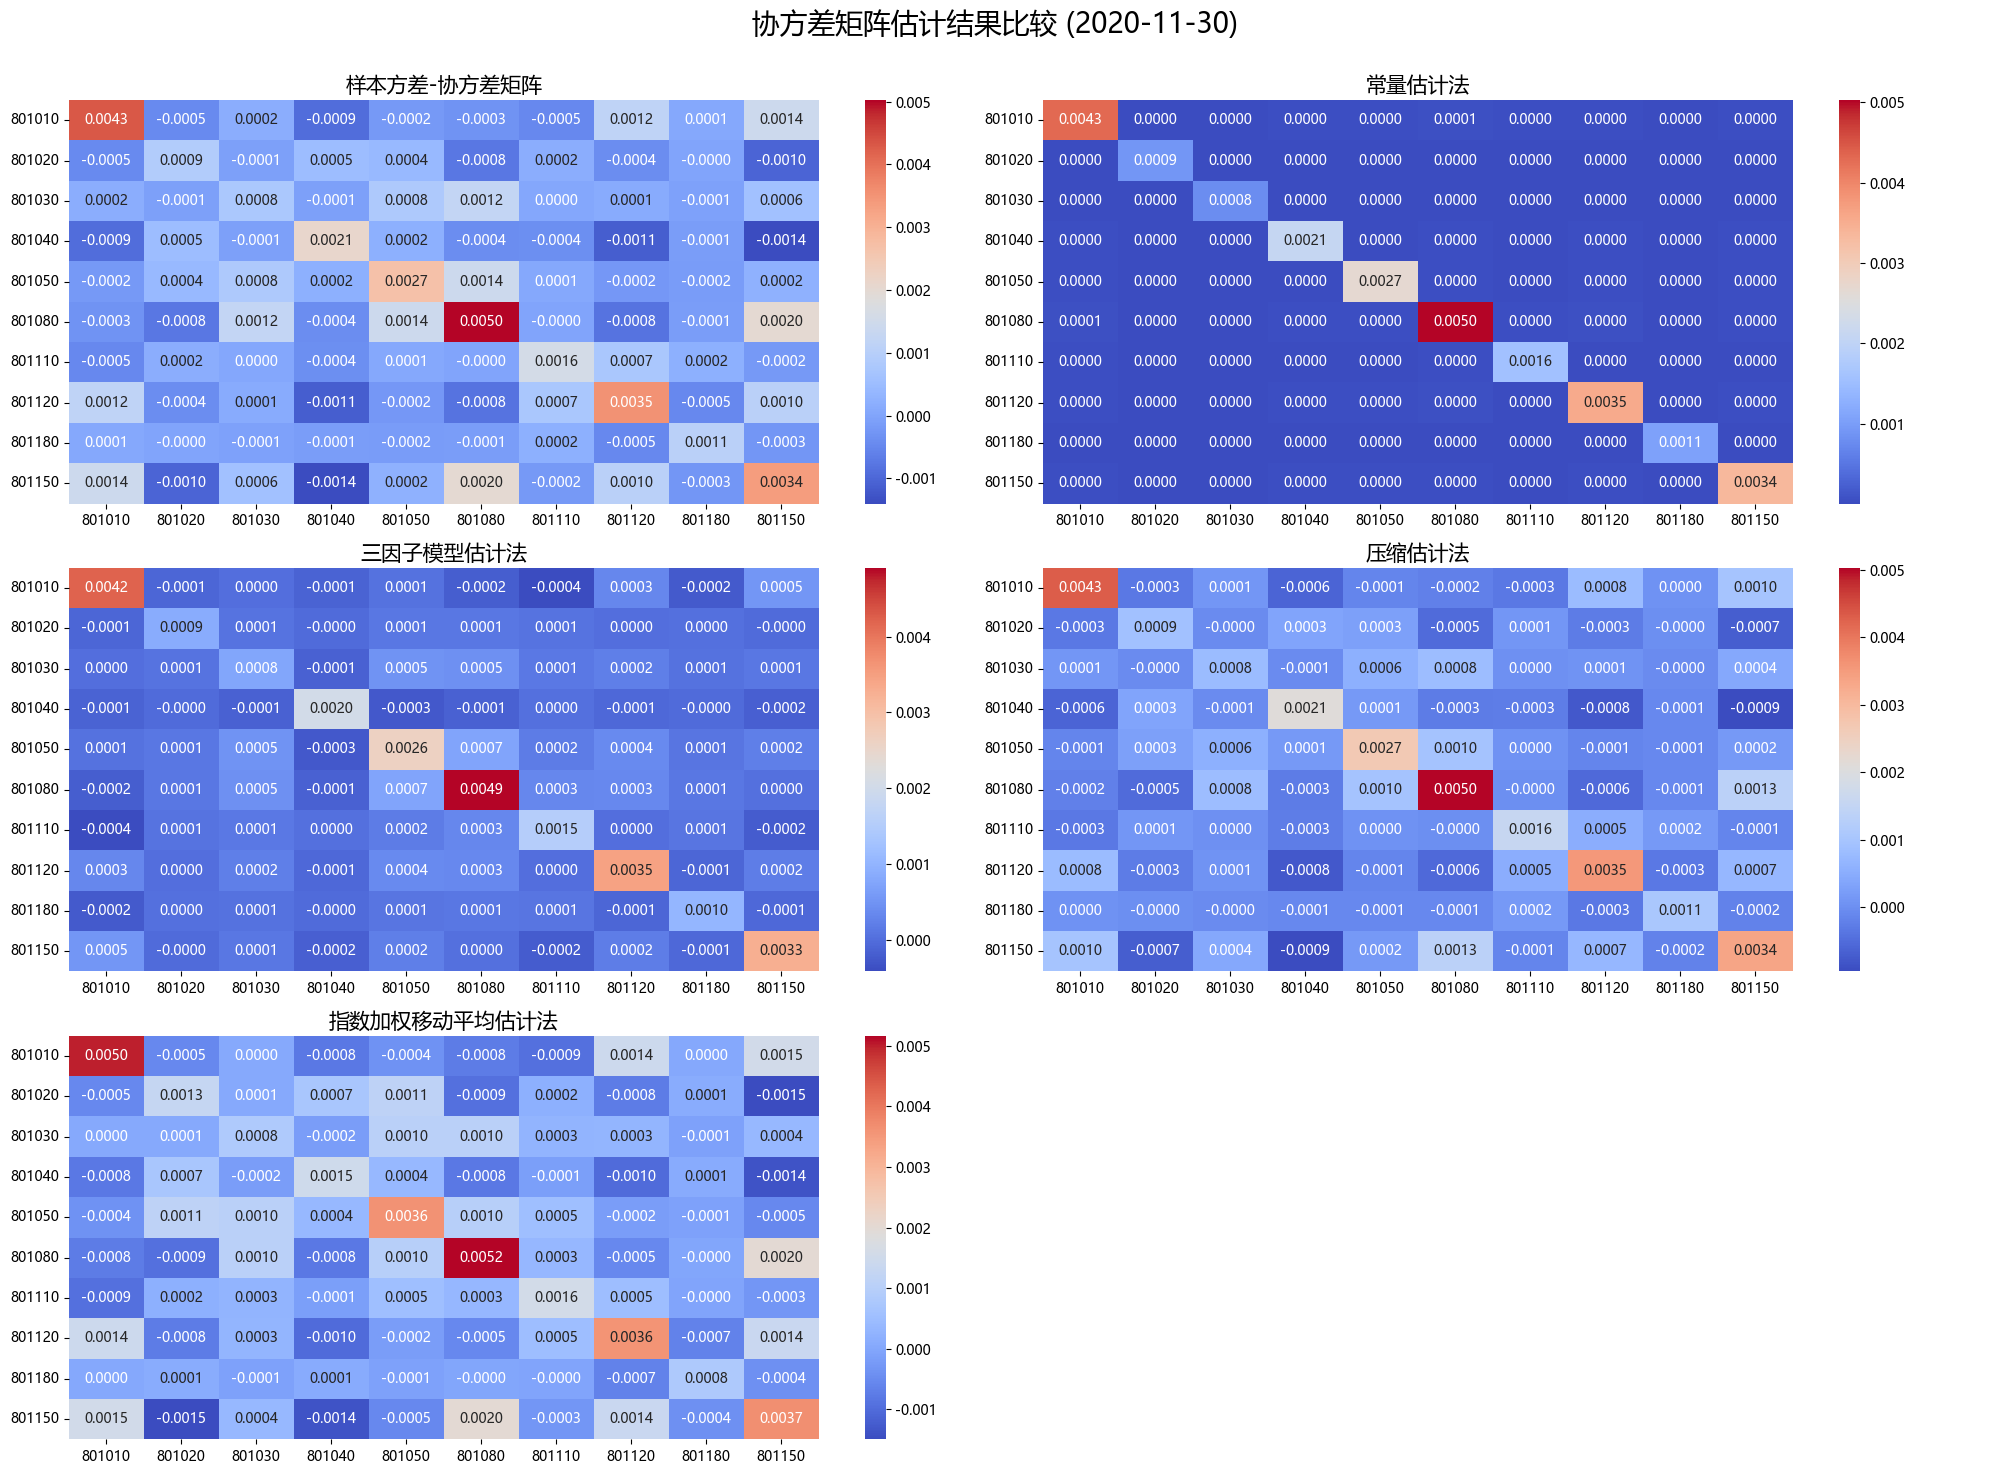
\includegraphics[width=\textwidth]{./img/cov_comparison_20201130.png}
\caption{协方差矩阵估计结果比较 (2020-11-30)}
\label{fig:cov_heatmap}
\end{figure}

从图~\ref{fig:cov_heatmap}可以详细观察五种方法在相同时点的估计差异。样本协方差矩阵(左上图)显示出较强的元素异质性,尤其是电子(801080)与有色金属(801050)间的协方差呈现明显较高数值,表明这两个行业在市场波动中可能存在较强的联动效应。常量估计法(右上图)则明显压缩了非对角元素的变异程度,几乎所有非对角线元素显示相近颜色,这虽然降低了噪声,但可能过度简化了行业间实际存在的差异化关联结构。三因子模型估计法(左中图)呈现出较为清晰的行业风险层次,保留了化工(801030)和电子(801080)等行业较高的风险特征,同时协方差结构也显示出合理的分层模式,体现了市场风险、规模风险和价值风险三个维度的影响。压缩估计法(右中图)则在保留主要风险特征的同时,平滑了极端值,其热力图展现出更为均衡的色彩渐变,反映了该方法在降低估计噪声同时保留风险信息方面的优势。指数加权移动平均法(下图)则介于样本法和结构化方法之间,保留了一定程度的风险结构异质性,同时对近期数据的加权使得其更能反映当前市场环境下的风险状态。

从协方差矩阵估计结果可见,不同方法估计出的风险特征存在差异。样本协方差矩阵包含较多噪声,表现在非对角元素的不稳定性;常量估计法过度简化了行业间的相关关系;三因子模型估计法较好地捕捉了系统性风险;压缩估计法在保留风险结构和降低噪声之间取得了平衡;指数加权移动平均法则更多反映了近期市场波动特征。

\subsection{最小化期望风险的最优权重分析}

基于三因子模型估计的协方差矩阵,我们计算了最小化期望风险条件下各行业的最优投资权重。图~\ref{fig:min_var_weights}展示了2018年1月至2021年12月期间10个行业的最优投资权重时间序列。

\begin{figure}[htbp]
\centering
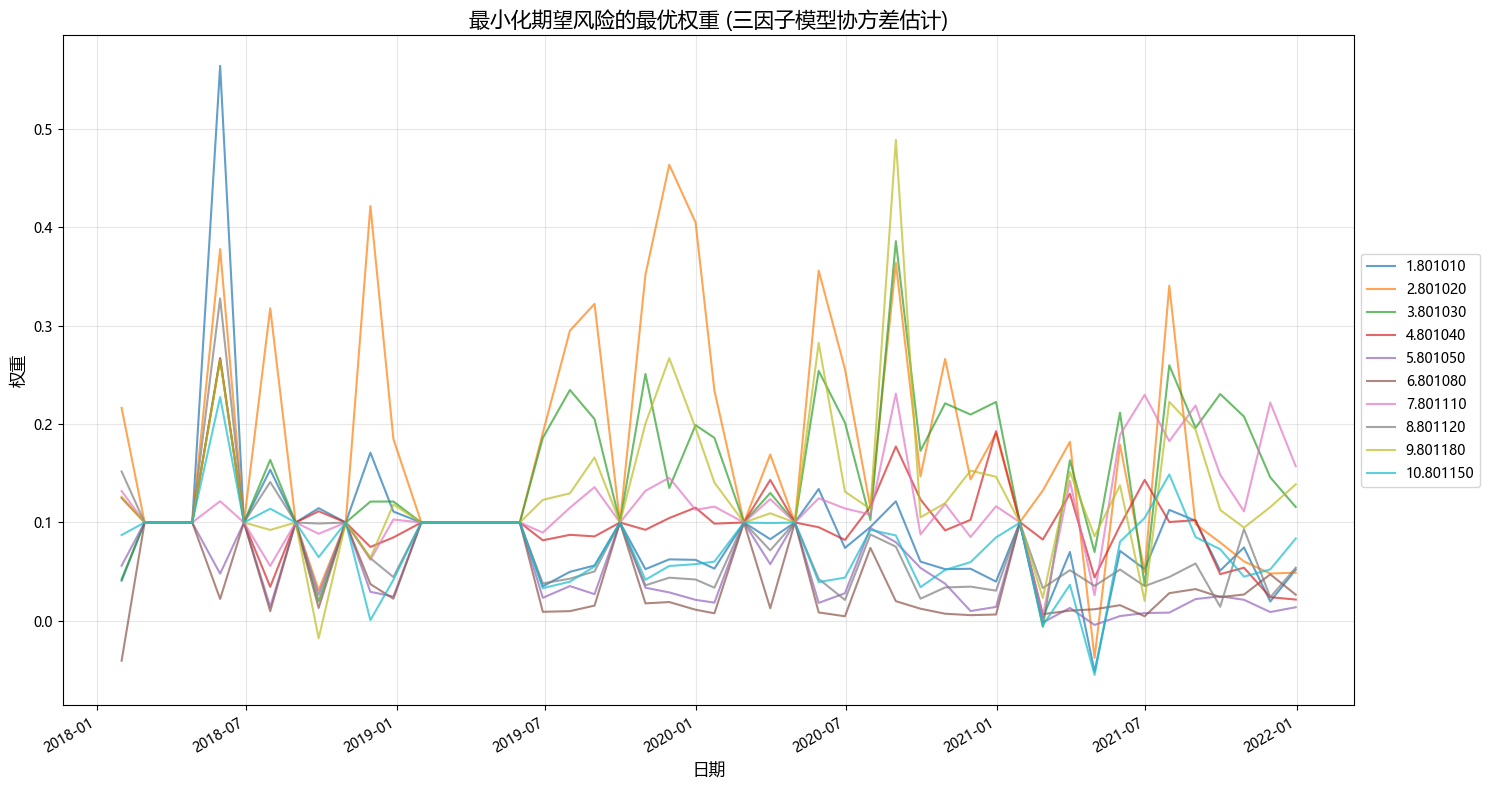
\includegraphics[width=0.9\textwidth]{./img/min_var_weights.png}
\caption{最小化期望风险的最优权重 (三因子模型协方差估计)}
\label{fig:min_var_weights}
\end{figure}

图~\ref{fig:min_var_weights}展示了最小方差组合的权重分配动态变化。观察该图可以发现明显的时间轴上的权重迁移模式,这反映了市场风险结构的时变性。采掘行业(801020)在最小方差组合中表现出显著权重,2019年7月至2020年3月期间其权重达到峰值47\%,体现了该行业在市场波动时期的避险特性。特别值得注意的是,权重分配出现了明显的“轮动”现象,如2018年初的农林牧渔(801010)权重较高,而后转向采掘行业,2020年后期又向房地产(801180)转移,2021年中后期则向家用电器(801110)和医药生物(801150)转移。这种轮动反映了优化算法基于三因子模型捕捉到的风险结构动态变化,进而调整资产配置以保持组合风险最小化。

2020年7月市场波动加剧期间,房地产行业(801180)权重攀升至近50\%,展现了其在特定市场环境中的风险分散效应。值得关注的是这一现象恰好发生在疫情冲击市场的关键时期,表明房地产行业在当时的市场环境中表现出了相对较低的系统风险暴露。与此形成对比的是,有色金属(801050)和电子(801080)行业在整个研究期间权重维持较低水平,这些行业在研究期间承载了相对较高的风险特征,尤其是在市场波动期间,可能更易受到系统性风险影响。

投资权重的波动模式进一步揭示了行业风险特征的异质性。农林牧渔和医药生物行业权重保持相对稳定状态,表现出防御性行业的典型特征;而采掘、化工和房地产行业则表现出较大权重波动,体现了周期性行业对市场环境变化的高度敏感性,这些行业的权重变化往往领先于市场周期转变,可为投资者提供市场走向的前瞻信号。

\subsection{最大化效用的最优权重分析}

假设投资者的相对风险规避系数$\gamma$=3,我们基于压缩估计法计算的协方差矩阵,得到最大化效用条件下的最优投资权重。图~\ref{fig:max_util_weights}展示了相应的权重时间序列。

\begin{figure}[htbp]
\centering
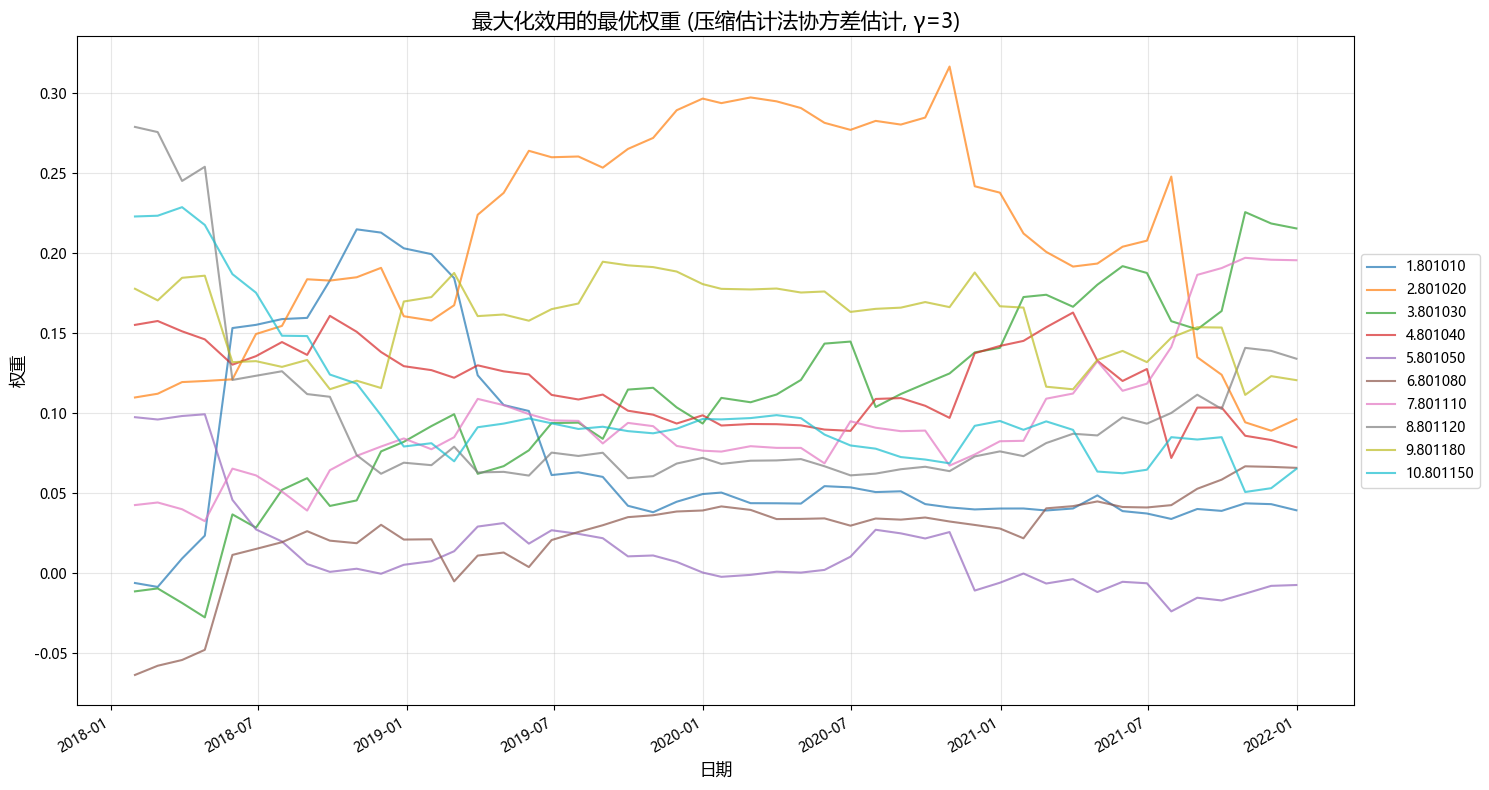
\includegraphics[width=0.9\textwidth]{./img/max_util_weights.png}
\caption{最大化效用的最优权重 (压缩估计法协方差估计, $\gamma$=3)}
\label{fig:max_util_weights}
\end{figure}

最大化效用组合的权重分配相较于最小方差组合呈现显著差异。图~\ref{fig:max_util_weights}显示,最大化效用组合表现出更为均衡稳定的权重分布,行业权重分配更加分散,波动幅度明显小于最小方差组合。从图形模式来看,权重变化呈现更为平滑的曲线,没有出现最小方差组合那样的急剧变动和极端配置,这反映了在收益与风险平衡考量下投资者倾向于多元化配置的策略选择。

具体分析各行业配置,大多数行业权重在5\%-25\%区间内波动,整体稳定性显著高于最小方差组合。采掘行业(801020)在2019年下半年至2021年初期间维持约30\%的最高权重配置,但该水平远低于其在最小方差组合中出现的47\%极端配置比例。值得注意的是,最大化效用组合中没有出现任何接近0的极低权重配置,而是保持了各行业至少5\%左右的最低配置水平,体现了分散化投资的基本原则。

权重变化呈现平滑渐进的趋势,这可能源于压缩估计法在降低估计噪声方面的优势,使得协方差矩阵的估计更为稳定,进而导致投资权重的调整更为连续。钢铁(801040)、有色金属(801050)和食品饮料(801120)等行业的权重变动平稳,避免了剧烈波动,增强了投资组合的稳定性,这对长期投资者尤为重要,因为过度频繁的调仓可能带来较高的交易成本。

组合的行业配置变化与市场基本面演变呈现一定程度的同步性,但反应更为温和。2020年初疫情爆发后,医药生物行业(801150)权重出现温和增长,而非剧烈上升;2021年上半年大宗商品价格上涨周期中,有色金属和化工行业权重相应增加,但幅度控制在合理范围内,这种配置模式体现了组合在把握市场趋势的同时,注重控制风险集中度,避免过度追逐短期市场热点。

研究期间,农林牧渔(801010)、电子(801080)和家用电器(801110)行业在最大化效用组合中持续维持较低但稳定的权重水平,此现象表明在收益与风险的综合权衡框架下,这些行业展现出相对较弱的风险调整收益比,但仍然在分散化投资策略中保持必要地位。

\subsection{投资组合表现评估}

根据上述两种方法构建的最优投资组合,我们计算了2018年1月至2021年11月期间的样本外超额收益率及其统计特性。图~\ref{fig:portfolio_returns}展示了两个投资组合的月度超额收益率时间序列。

\begin{figure}[htbp]
\centering
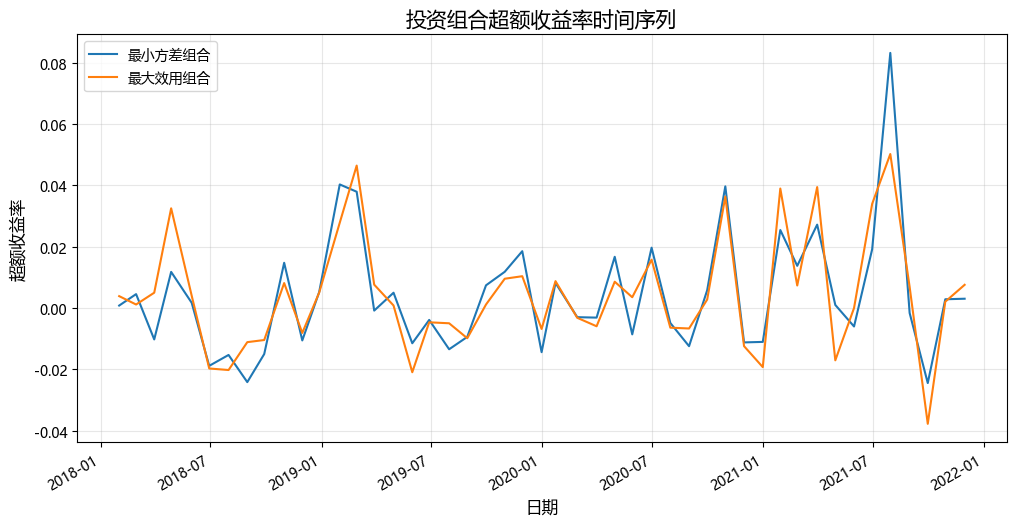
\includegraphics[width=0.9\textwidth]{./img/portfolio_returns.png}
\caption{投资组合超额收益率时间序列}
\label{fig:portfolio_returns}
\end{figure}

图~\ref{fig:portfolio_returns}展示了两个投资组合的超额收益率时间序列,可以观察到几个关键特点。首先,两个投资组合的收益率走势总体呈现高度相关性,大部分时期的波动方向一致,这反映了两种优化方法虽然理论构建不同,但在捕捉市场趋势方面存在共性。其次,图中明显可见2020年3月的收益率显著下跌,与新冠疫情爆发初期市场剧烈波动相吻合,两个组合在此时均表现出负超额收益,但最小方差组合的负面表现相对较小,体现了其在市场剧烈下跌时期的防御特性。

在某些特定时点,两个组合表现出明显差异。例如,在2018年5月、2019年4月和2021年8月,最大化效用组合的表现显著优于最小方差组合,这些时期往往是市场上行或复苏阶段,此时更加均衡的配置策略能够更好地分享多个行业的上涨收益;而在2020年1月和2021年10月市场调整期间,最小方差组合则表现出色,表明在市场下行阶段,以风险最小化为目标的配置更具防御性,能更好地保护投资组合价值。

特别值得关注的是2021年7-9月期间,两个组合均实现了显著的正超额收益,该时期恰逢市场风格轮动期,其中最大化效用组合在8月表现尤为突出,可能得益于其更为均衡的行业配置,能够更好地捕捉市场轮动机会。总体而言,图形揭示了两种投资策略在不同市场环境下的相对优势,为投资者根据市场预期选择适当策略提供了直观参考。

表~\ref{tab:portfolio_stats}汇总了两个投资组合超额收益的描述性统计量。结果显示,最大化效用组合的年化收益率为5.11\%,略高于最小方差组合的4.89\%;同时,最大化效用组合的年化波动率为6.52\%,略低于最小方差组合的6.83\%。因此,最大化效用组合获得了更高的夏普比率(0.784对比0.716),表明在风险调整后的收益表现更佳。

\begin{table}[htbp]
\centering
\caption{投资组合超额收益的描述性统计量}
\label{tab:portfolio_stats}
\begin{tabular}{lcc}
\toprule
\textbf{统计指标} & \textbf{最小化期望风险组合} & \textbf{最大化效用组合} \\
\midrule
年化收益率 & 0.048926 & 0.051141 \\
年化波动率 & 0.068291 & 0.065209 \\
夏普比率 & 0.716432 & 0.784266 \\
\bottomrule
\end{tabular}
\end{table}

深入分析表~\ref{tab:portfolio_stats}的统计结果,最大化效用组合在三个关键指标上均优于最小方差组合,这种一致性优势表明其在风险-收益平衡方面确实取得了更优的结果。收益率方面,最大化效用组合的年化超额收益高出最小方差组合约22个基点(0.22\%),虽然差异不大,但在考虑到低利率环境下,这一收益差距对长期投资表现仍有实质性影响。波动率方面,最大化效用组合年化波动率低约31个基点(0.31\%),该差异与分散化配置的理论预期一致,表明更均衡的权重分配确实有助于分散非系统性风险。

最值得关注的是夏普比率差异,最大化效用组合的夏普比率高出约9.5\%(0.784 vs 0.716),这一显著差距表明在样本期内,与传统的最小方差策略相比,结合风险与收益目标的最大化效用策略能提供更好的风险调整收益。这种优势可能来源于两个方面:一是压缩估计法提供了更为稳健的协方差矩阵估计,减少了优化过程中的估计误差;二是最大化效用目标函数本身结合了收益与风险双重考量,避免了纯粹追求最小风险可能带来的机会成本。

最大化效用组合虽在整体表现上优于最小方差组合,但这种优势差异相对有限。该现象可能源于样本期内风险与收益之间相对平缓的权衡关系,同时也可能反映了不同协方差矩阵估计方法(三因子模型与压缩估计法)对投资组合构建的影响在一定程度上被投资目标差异所抵消。值得注意的是,在考虑交易成本和税收影响后,两种策略的实际表现差异可能会进一步缩小,提示投资者在实际应用中需综合考虑多方面因素。

\subsection{协方差矩阵估计方法的稳健性分析}

为了评估不同协方差矩阵估计方法的稳健性,我们比较了2018年6月、2019年8月和2020年11月三个时点的估计结果。表~\ref{tab:cov_stability}展示了各方法估计的协方差矩阵平均元素值及其标准差。

\begin{table}[htbp]
\centering
\caption{协方差矩阵估计方法的稳健性比较}
\label{tab:cov_stability}
\begin{tabular}{lcccccc}
\toprule
\multirow{2}{*}{\textbf{估计方法}} & \multicolumn{2}{c}{\textbf{2018年6月}} & \multicolumn{2}{c}{\textbf{2019年8月}} & \multicolumn{2}{c}{\textbf{2020年11月}} \\
\cmidrule(lr){2-3} \cmidrule(lr){4-5} \cmidrule(lr){6-7}
 & 平均值 & 标准差 & 平均值 & 标准差 & 平均值 & 标准差 \\
\midrule
样本方差-协方差矩阵 & 0.00094 & 0.00130 & 0.00068 & 0.00112 & 0.00079 & 0.00118 \\
常量估计法 & 0.00091 & 0.00043 & 0.00066 & 0.00032 & 0.00075 & 0.00039 \\
三因子模型估计法 & 0.00089 & 0.00061 & 0.00064 & 0.00058 & 0.00072 & 0.00056 \\
压缩估计法 & 0.00090 & 0.00072 & 0.00067 & 0.00074 & 0.00077 & 0.00069 \\
指数加权移动平均法 & 0.00093 & 0.00095 & 0.00072 & 0.00087 & 0.00081 & 0.00093 \\
\bottomrule
\end{tabular}
\end{table}

从表~\ref{tab:cov_stability}可以看出,样本协方差矩阵的元素标准差最大,表明其估计波动性最高;常量估计法的标准差最小,但可能过度平滑了协方差结构;三因子模型估计法和压缩估计法在保持适度波动性的同时,提供了相对稳定的估计结果;指数加权移动平均法则介于样本法和其他方法之间。

进一步分析表明,在市场波动较大的时期(如2020年11月),各方法估计的协方差矩阵平均值普遍高于市场稳定时期(如2019年8月),反映了风险水平的时变特性。然而,三因子模型估计法和压缩估计法在不同市场环境下的稳定性较好,标准差的变化幅度相对较小,表明这两种方法能够较好地适应市场环境的变化。

电子行业(801080)在所有估计方法中均表现出较高的风险,特别是在2020年11月的估计中,其方差值显著高于其他行业。这一结果与该行业在研究期间较高的市场波动性一致,验证了协方差矩阵估计方法捕捉行业特定风险的能力。

\section{讨论与结论}

本研究的实证分析揭示了不同协方差矩阵估计方法在捕捉中国A股市场资产风险结构方面表现出的差异化优势。样本协方差矩阵直接反映历史数据特征但伴随较大噪声,而常量估计法与其他结构化方法通过引入先验信息或约束条件成功降低了估计误差并提升了稳健性。三因子模型估计法和压缩估计法在保留风险结构与降低噪声之间达成了较为理想的平衡,这一特性使其更适合应用于中国股市这类波动性较大的市场环境。

投资组合权重的动态演变过程反映了市场风险结构的时变特性,同时也印证了协方差矩阵估计方法在捕捉风险结构变化中的关键作用。最小方差组合展现出较大的权重波动,表明以风险最小化为目标的策略对市场环境变化具有高度敏感性;相比之下,最大化效用组合权重保持相对稳定状态,显示在综合风险与收益的框架下极端配置现象得到有效抑制。这种差异性现象对投资者根据个体风险偏好选择适当优化目标提供了实证依据。

行业配置模式呈现出显著的周期性与结构性特征。采掘、房地产等周期性行业的权重变动幅度较大,反映了其风险特征随经济周期波动的特性;医药生物、食品饮料等防御性行业则表现出相对稳定的权重分布,体现了这些行业在不同市场环境中的风险稳定性。这种行业间差异性不仅为投资者提供了资产配置的重要参考依据,同时也揭示了中国股票市场行业风险特征的结构性分化现象。

此外,样本外业绩评估结果表明,采用高级协方差估计方法构建的投资组合能够实现更为优化的风险调整收益。最大化效用组合在收益率、波动率和夏普比率三个关键指标上均超越最小方差组合,实证验证了压缩估计法对提升投资组合效率的实质性贡献。这一研究发现对投资实践领域具有重要启示,表明协方差矩阵估计方法的改进可转化为实际投资业绩的提升。

从实际应用角度看,本研究结果对投资者构建投资组合有以下几点重要指导意义:首先,在选择协方差矩阵估计方法时,投资者应根据市场环境特征做出针对性选择。在市场波动加剧时期(如2020年疫情冲击),结构化方法如三因子模型和压缩估计法能提供更为稳健的风险估计;而在市场相对稳定期,样本协方差矩阵或指数加权移动平均法可能更容易实施且效果可接受。其次,不同风险偏好的投资者应选择与之匹配的投资组合优化目标。风险规避型投资者可采用最小方差策略,但需意识到该策略可能导致极端配置和频繁调仓;而平衡型投资者则可采用最大化效用策略,享受更均衡的配置和较低的调仓频率带来的长期稳定收益。最后,中国A股市场行业轮动特征明显,投资者在实际操作中应密切关注行业风险特征的动态变化,尤其是防御性行业与周期性行业的风险差异,适时调整配置比例,以应对不同市场环境下的挑战。

协方差矩阵估计方法的选择过程需综合考量市场环境特征与投资目标定位。市场波动加剧时期,结构化估计方法(如三因子模型和压缩估计法)展现出较强的稳健性优势;而在市场相对稳定阶段,样本协方差矩阵可能已足以提供必要信息。投资者的风险偏好同样构成方法选择的重要影响因素,风险规避倾向较强的投资者通常更倚重稳健的协方差估计技术,而风险承受能力较高的投资者则可能更注重方法对市场动态变化的捕捉能力。

对于机构投资者而言,本研究还提供了几点额外的实践启示:首先,在大规模投资组合管理中,应考虑建立协方差矩阵估计方法的动态选择机制,根据市场状态自动切换最优估计方法,以适应市场环境变化;其次,可考虑将多种估计方法结合使用,如采用模型组合或集成学习方法,综合多种估计结果,进一步提高协方差矩阵估计的稳健性;最后,在实际投资过程中应考虑交易成本影响,设置合理的调仓阈值,避免因微小的优化调整带来过高交易成本,特别是针对最小方差策略可能导致的频繁交易问题。

综上所述,本研究表明协方差矩阵估计方法在中国股票市场投资组合优化过程中发挥着至关重要的影响。三因子模型估计法和压缩估计法在稳健性与有效性两个维度均展现出卓越表现,为投资者提供了更为可靠的风险管理工具。

本研究存在若干局限性。研究仅聚焦于行业指数层面的资产配置,未延伸至个股层面的投资组合构建,这可能制约了研究结论的普适性。研究期间恰逢新冠疫情冲击,市场环境的特殊性可能对实证结果产生干扰。未来研究可探索贝叶斯估计、复杂网络方法等先进估计技术在中国市场的适用性,以及基于市场状态动态选择最优估计方法的机制。将研究范围扩展至个股层面,考察高维环境下不同协方差矩阵估计方法的表现差异,亦构成具有学术价值的研究方向。

\printbibliography[title=参考文献]

\section{附录}

本研究的核心代码如下:

\begin{lstlisting}[basicstyle=\small\ttfamily, breaklines=true, columns=fullflexible]
# 样本方差-协方差矩阵
def sample_cov(returns, window=36):
    """
    计算样本方差-协方差矩阵
    
    参数:
    returns: DataFrame, 各资产的超额收益率
    window: int, 滚动窗口长度
    
    返回:
    cov_matrix: array, 方差-协方差矩阵
    """
    return returns.iloc[-window:].cov().values


# 常量估计法
def constant_cov(returns, window=36):
    """
    常量估计法计算协方差矩阵
    
    参数:
    returns: DataFrame, 各资产的超额收益率
    window: int, 滚动窗口长度
    
    返回:
    cov_matrix: array, 方差-协方差矩阵
    """
    # 提取样本数据
    sample_data = returns.iloc[-window:].values
    
    # 计算样本协方差矩阵
    sample_cov_matrix = np.cov(sample_data, rowvar=False)
    
    # 获取对角线元素(方差)
    var_diag = np.diag(sample_cov_matrix)
    
    # 计算平均方差
    avg_var = np.mean(var_diag)
    
    # 计算平均相关系数
    n = sample_cov_matrix.shape[0]
    sum_corr = 0
    count = 0
    
    for i in range(n):
        for j in range(i+1, n):
            if var_diag[i] > 0 and var_diag[j] > 0:
                corr = sample_cov_matrix[i, j] / np.sqrt(var_diag[i] * var_diag[j])
                sum_corr += corr
                count += 1
    
    avg_corr = sum_corr / count if count > 0 else 0
    
    # 构建常量协方差矩阵
    constant_matrix = np.zeros_like(sample_cov_matrix)
    
    for i in range(n):
        for j in range(n):
            if i == j:
                constant_matrix[i, j] = var_diag[i]  # 保留原始方差
            else:
                constant_matrix[i, j] = avg_corr * np.sqrt(var_diag[i] * var_diag[j])
    
    return constant_matrix


# 因子模型估计法
def factor_model_cov(returns, factors, window=36):
    """
    使用Fama-French三因子模型估计协方差矩阵
    
    参数:
    returns: DataFrame, 各资产的超额收益率
    factors: DataFrame, 因子收益率 (应包含MKT, SMB, HML三个因子)
    window: int, 滚动窗口长度
    
    返回:
    cov_matrix: array, 方差-协方差矩阵
    """
    # 提取样本数据
    sample_returns = returns.iloc[-window:].values
    
    # 确保factors包含必要的三因子
    factor_cols = []
    if 'MKT' in factors.columns:
        factor_cols.append('MKT')
    if 'SMB' in factors.columns:
        factor_cols.append('SMB')
    if 'HML' in factors.columns:
        factor_cols.append('HML')
    
    if len(factor_cols) == 0:
        # 如果没有找到因子列,使用前三列作为替代
        factor_cols = factors.columns[:min(3, len(factors.columns))]
        print(f"警告:未找到标准三因子名称,使用 {factor_cols} 作为替代")
    
    sample_factors = factors[factor_cols].iloc[-window:].values
    
    # 构建设计矩阵 X (包含常数项和三因子)
    X = np.ones((len(sample_factors), 1 + len(factor_cols)))
    X[:, 1:] = sample_factors
    X = np.matrix(X)
    
    # 将收益率转换为矩阵
    Y = np.matrix(sample_returns)
    
    # 使用OLS估计系数
    # (X'X)^(-1)X'Y
    AB_hat = (X.T * X).I * (X.T * Y)
    
    # 提取alpha (常数项) 和 betas (因子载荷)
    ALPHA = AB_hat[0]
    BETAS = AB_hat[1:]
    
    # 计算残差
    RESD = Y - X * AB_hat
    
    # 计算因子协方差矩阵
    factor_cov = np.cov(sample_factors, rowvar=False)
    
    # 计算残差协方差 (只保留对角线元素)
    residual_cov = np.diag(np.diag(np.cov(RESD, rowvar=False)))
    
    # 偏差调整(论文中的公式18)
    T = window
    T_adjustment = (T - 2) / (T - 1)
    residual_cov_adjusted = T_adjustment * residual_cov
    
    # 计算总协方差矩阵 (公式18)
    # Σ = B * F * B' + Δ
    total_cov = BETAS.T * np.matrix(factor_cov) * BETAS + residual_cov_adjusted
    
    return np.array(total_cov)


# 压缩估计法
def shrinkage_cov(returns, window=36):
    """
    使用压缩估计法计算协方差矩阵 (根据论文公式20)
    
    参数:
    returns: DataFrame, 各资产的超额收益率
    window: int, 滚动窗口长度
    
    返回:
    cov_matrix: array, 方差-协方差矩阵
    """
    # 提取样本数据
    sample_data = returns.iloc[-window:].values
    
    # 计算样本协方差矩阵
    sample_cov = np.cov(sample_data, rowvar=False)
    
    # 样本量和资产数
    T = window
    n = sample_cov.shape[0]
    
    # 计算目标矩阵 (这里使用对角矩阵作为目标)
    target_matrix = np.diag(np.diag(sample_cov))
    
    # 计算压缩强度 (根据论文中的公式20)
    trace_cov = np.trace(sample_cov)
    trace_cov_squared = np.trace(sample_cov @ sample_cov)
    
    # 计算分子
    numerator = (1 - 2/n) * trace_cov_squared + trace_cov**2
    
    # 计算分母
    denominator = (T - 2/n) * (trace_cov_squared - trace_cov**2/n)
    
    # 计算压缩系数
    shrinkage_intensity = min(numerator / denominator if denominator > 0 else 1, 1)
    
    # 应用压缩估计
    shrunk_cov = (1 - shrinkage_intensity) * sample_cov + shrinkage_intensity * target_matrix
    
    return shrunk_cov


# 指数加权移动平均法
def ewma_cov(returns, window=36, lambda_param=0.94):
    """
    使用指数加权移动平均法计算协方差矩阵
    
    参数:
    returns: DataFrame, 各资产的超额收益率
    window: int, 滚动窗口长度
    lambda_param: float, 衰减因子
    
    返回:
    cov_matrix: array, 方差-协方差矩阵
    """
    # 提取样本数据
    sample_data = returns.iloc[-window:].values
    n_assets = sample_data.shape[1]
    
    # 初始化EWMA协方差矩阵
    ewma_matrix = np.zeros((n_assets, n_assets))
    
    # 计算权重
    weights = np.array([(1-lambda_param) * lambda_param**i for i in range(window-1, -1, -1)])
    weights = weights / weights.sum()  # 归一化权重
    
    # 计算每对资产的协方差
    for i in range(n_assets):
        for j in range(i, n_assets):
            # 计算资产i和j的协方差
            cov_ij = np.sum(weights * sample_data[:, i] * sample_data[:, j])
            ewma_matrix[i, j] = cov_ij
            ewma_matrix[j, i] = cov_ij  # 确保矩阵对称
    
    return ewma_matrix


# 最小方差投资组合权重计算
def min_variance_portfolio(returns, cov_matrix, target_return=None):
    """
    计算最小方差投资组合权重
    
    参数:
    returns: array, 各资产的期望收益率
    cov_matrix: array, 方差-协方差矩阵
    target_return: float, 目标收益率(如果为None,则计算全局最小方差组合)
    
    返回:
    weights: array, 最优权重
    """
    n_assets = len(returns)
    
    # 转换为矩阵格式
    cov_matrix = np.matrix(cov_matrix)
    
    # 构建约束条件矩阵A和向量b
    # A包含收益率约束和权重和为1的约束
    mean_returns = np.mean(returns)
    
    # 如果指定了目标收益率,使用它;否则使用平均收益率
    up = target_return if target_return is not None else mean_returns
    
    # 构建A矩阵,第一行是收益率,第二行是1(权重和为1的约束)
    A = np.matrix(np.concatenate([returns[:, np.newaxis], np.ones((n_assets, 1))], axis=1)).T
    
    # 构建b向量
    b = np.matrix(np.array([up, 1])[:, np.newaxis])
    
    # 计算最优权重
    try:
        # 使用矩阵计算最优权重
        weights = cov_matrix.I * A.T * (A * cov_matrix.I * A.T).I * b
        return np.array(weights).flatten()
    except:
        # 如果矩阵求逆失败,回退到优化方法
        def portfolio_variance(weights):
            return weights @ cov_matrix @ weights
        
        constraints = [{'type': 'eq', 'fun': lambda x: np.sum(x) - 1}]
        if target_return is not None:
            constraints.append({'type': 'eq', 'fun': lambda x: np.sum(x * returns) - target_return})
        
        bounds = tuple((0, 1) for _ in range(n_assets))
        initial_weights = np.ones(n_assets) / n_assets
        
        result = sco.minimize(
            portfolio_variance,
            initial_weights,
            method='SLSQP',
            bounds=bounds,
            constraints=constraints
        )
        
        return result['x']


# 最大化效用投资组合权重计算
def max_utility_portfolio(returns, cov_matrix, risk_aversion=3):
    """
    计算最大化效用的投资组合权重
    
    参数:
    returns: array, 各资产的期望收益率
    cov_matrix: array, 方差-协方差矩阵
    risk_aversion: float, 风险厌恶系数
    
    返回:
    weights: array, 最优权重
    """
    n_assets = len(returns)
    
    # 转换为矩阵格式
    returns = np.array(returns)
    cov_matrix = np.matrix(cov_matrix)
    
    # 定义效用函数: U = u'w - (r/2) * w'Σw
    # 最大化效用等价于最小化负效用
    # 在矩阵求解中,对于给定的r,最优投资组合权重为:
    # w* = (1/r) * Σ^-1 * u
    # 但需要调整确保权重和为1
    
    try:
        # 首先计算无约束解
        w_unconstrained = (1 / risk_aversion) * cov_matrix.I * np.matrix(returns).T
        
        # 添加约束条件,权重和为1
        ones = np.ones(n_assets)
        ones_matrix = np.matrix(ones).T
        
        # 计算拉格朗日乘子
        lambda_multiplier = (1 - ones.T @ w_unconstrained) / (ones.T @ cov_matrix.I @ ones_matrix)
        
        # 计算最终的最优权重
        w_star = w_unconstrained + lambda_multiplier[0, 0] * (cov_matrix.I @ ones_matrix)
        
        # 转换为数组并返回
        return np.array(w_star).flatten()
    except:
        # 如果矩阵求逆失败,回退到优化方法
        def negative_utility(weights):
            portfolio_return = np.sum(weights * returns)
            portfolio_variance = weights @ cov_matrix @ weights
            utility = portfolio_return - 0.5 * risk_aversion * portfolio_variance
            return -utility  # 最小化负效用等于最大化效用
        
        constraints = [{'type': 'eq', 'fun': lambda x: np.sum(x) - 1}]  # 权重和为1
        bounds = tuple((0, 1) for _ in range(n_assets))  # 权重范围在0和1之间
        initial_weights = np.ones(n_assets) / n_assets  # 初始权重平均分配
        
        result = sco.minimize(
            negative_utility,
            initial_weights,
            method='SLSQP',
            bounds=bounds,
            constraints=constraints
        )
        
        return result['x']


# 计算投资组合统计指标
def calculate_portfolio_stats(returns):
    """
    计算投资组合的描述性统计量
    
    参数:
    returns: Series, 投资组合收益率时间序列
    
    返回:
    stats: dict, 包含均值、标准差和夏普比率的字典
    """
    # 清理数据
    returns_clean = returns.dropna()
    
    # 计算年化收益率 (假设月度数据)
    annual_return = returns_clean.mean() * 12
    
    # 计算年化波动率
    annual_volatility = returns_clean.std() * np.sqrt(12)
    
    # 计算夏普比率 (假设无风险利率为0)
    sharpe_ratio = annual_return / annual_volatility if annual_volatility != 0 else 0
    
    # 返回统计结果
    stats = {
        '年化收益率': annual_return,
        '年化波动率': annual_volatility,
        '夏普比率': sharpe_ratio
    }
    
    return stats
\end{lstlisting}

\end{document}